\documentclass[11pt]{jsarticle}

  % https://joker.hatenablog.com/entry/2012/07/09/153537
\usepackage[top=20truemm,bottom=30truemm,left=25truemm,right=25truemm]{geometry}
  % A4タテで,上2cm,下3cm,左右各2.5cmの余白をとる.
  % 用紙の左上4cm×4cmには講演番号が入るため,ここに文字がかぶらないようにする.

	% 図
\usepackage{graphicx}	% 画像読み込み
\usepackage{mediabb}	% 画像読み込み
\usepackage{wrapfig}	% 回りこみの画像

	% UDフォント
\usepackage{pxchfon}
\setminchofont{UDDIGIKYOKASHON-R.TTC} 
\setgothicfont{UDDIGIKYOKASHON-B.TTC} 

\pagestyle{empty}

\begin{document}
\Large

  % \begin{center}
  % \end{center}
\centerline{植生調査を支援するアプリの開発}

 \\[-12mm]

\normalsize
\rightline{松村俊和(甲南女子大学)}

 \\[-8mm]

\noindent
\textbf{[背景]}
植生調査をはじめとした生物の現地調査では,長年にわたって紙の調査票への記入が行われている.
紙への記入は,簡便,汎用性の高さ,文字情報以外も容易に記入可能といった多くの利点がある.
一方で,手作業での被度計算,目視による確認,PCへの記入データの入力などの欠点がある.

\noindent
\textbf{[目的]}
紙媒体の欠点を補えれば,植生調査の時間短縮や効率化に寄与できる可能性がある.
そこで植生調査を支援するアプリの開発に着手した.
紙媒体の欠点を補うとともに,以下の点を考慮した.
\vspace{-0.5\baselineskip}
\begin{itemize}
\item 汎用性の高いものとする(項目の設定・保存・復元が可能,植生調査以外でも利用可能).
\item OS・端末によらず利用可能(シェアの高いブラウザで動作).
\item 独立して動作可能(オフラインで動作可能,外部ライブラリやフレームワークは不使用).
\item 使用者が機能を追加・修正可能(ソースコードの公開).
\end{itemize}
\vspace{-0.5\baselineskip}

\noindent
\textbf{[使用言語等]}
HTML, JavaScript, CSS (HTMLにJavaScripとCSSを格納)

\noindent
\textbf{[動作確認環境]}
GoogleChrome 105.0.5195.102

\noindent
\textbf{[入手・起動]}
HTMLをダウンロード([Ctrl] + [S] - [ウェブページ,HTMLのみ])して,起動する.\\
https://matutosi.github.io/biodiv/biss.html

\noindent
\textbf{[使用方法]}

\noindent
\textbf{項目の設定(Settings):}
地点情報と観察情報の項目を設定する.
既定値では地点情報にPlot, Investigator, Date, Location, GPSデータ,階層データなど,
観察情報にDate,GPSデータ,Layer,Species, Coverなどがある,
それぞれを設定後,"Make plot table"を選択する.

\noindent
\textbf{データ入力(Inputs):}
地点情報を入力後"New occ table"で,観察情報の入力表が表示される.
観察情報ではテキストの検索,並び替え,列の表示・非表示,GPSデータの更新などが可能である.

\noindent
\textbf{和名検索(Tools):}
wameiに全角カタカナを入力,"Search text"で,該当和名が表示される.

\noindent
\textbf{[出力形式]}
設定ファイルおよび入力データともに,列名・データ形式・選択リスト・データの4項目からなるテキストファイルである.
各項目はJSON形式であり,";"(セミコロン)で区切られている.
出力データは電子メールの添付ファイルとして送信する.
Rではテキストファイルを読み込み,";"で区切れば,jsonlite等のパッケージを使ってデータフレームへの変換ができる.
筆者作成の関数(ecan::read\_biss())も利用可能である.

\vspace{5mm}
\noindent
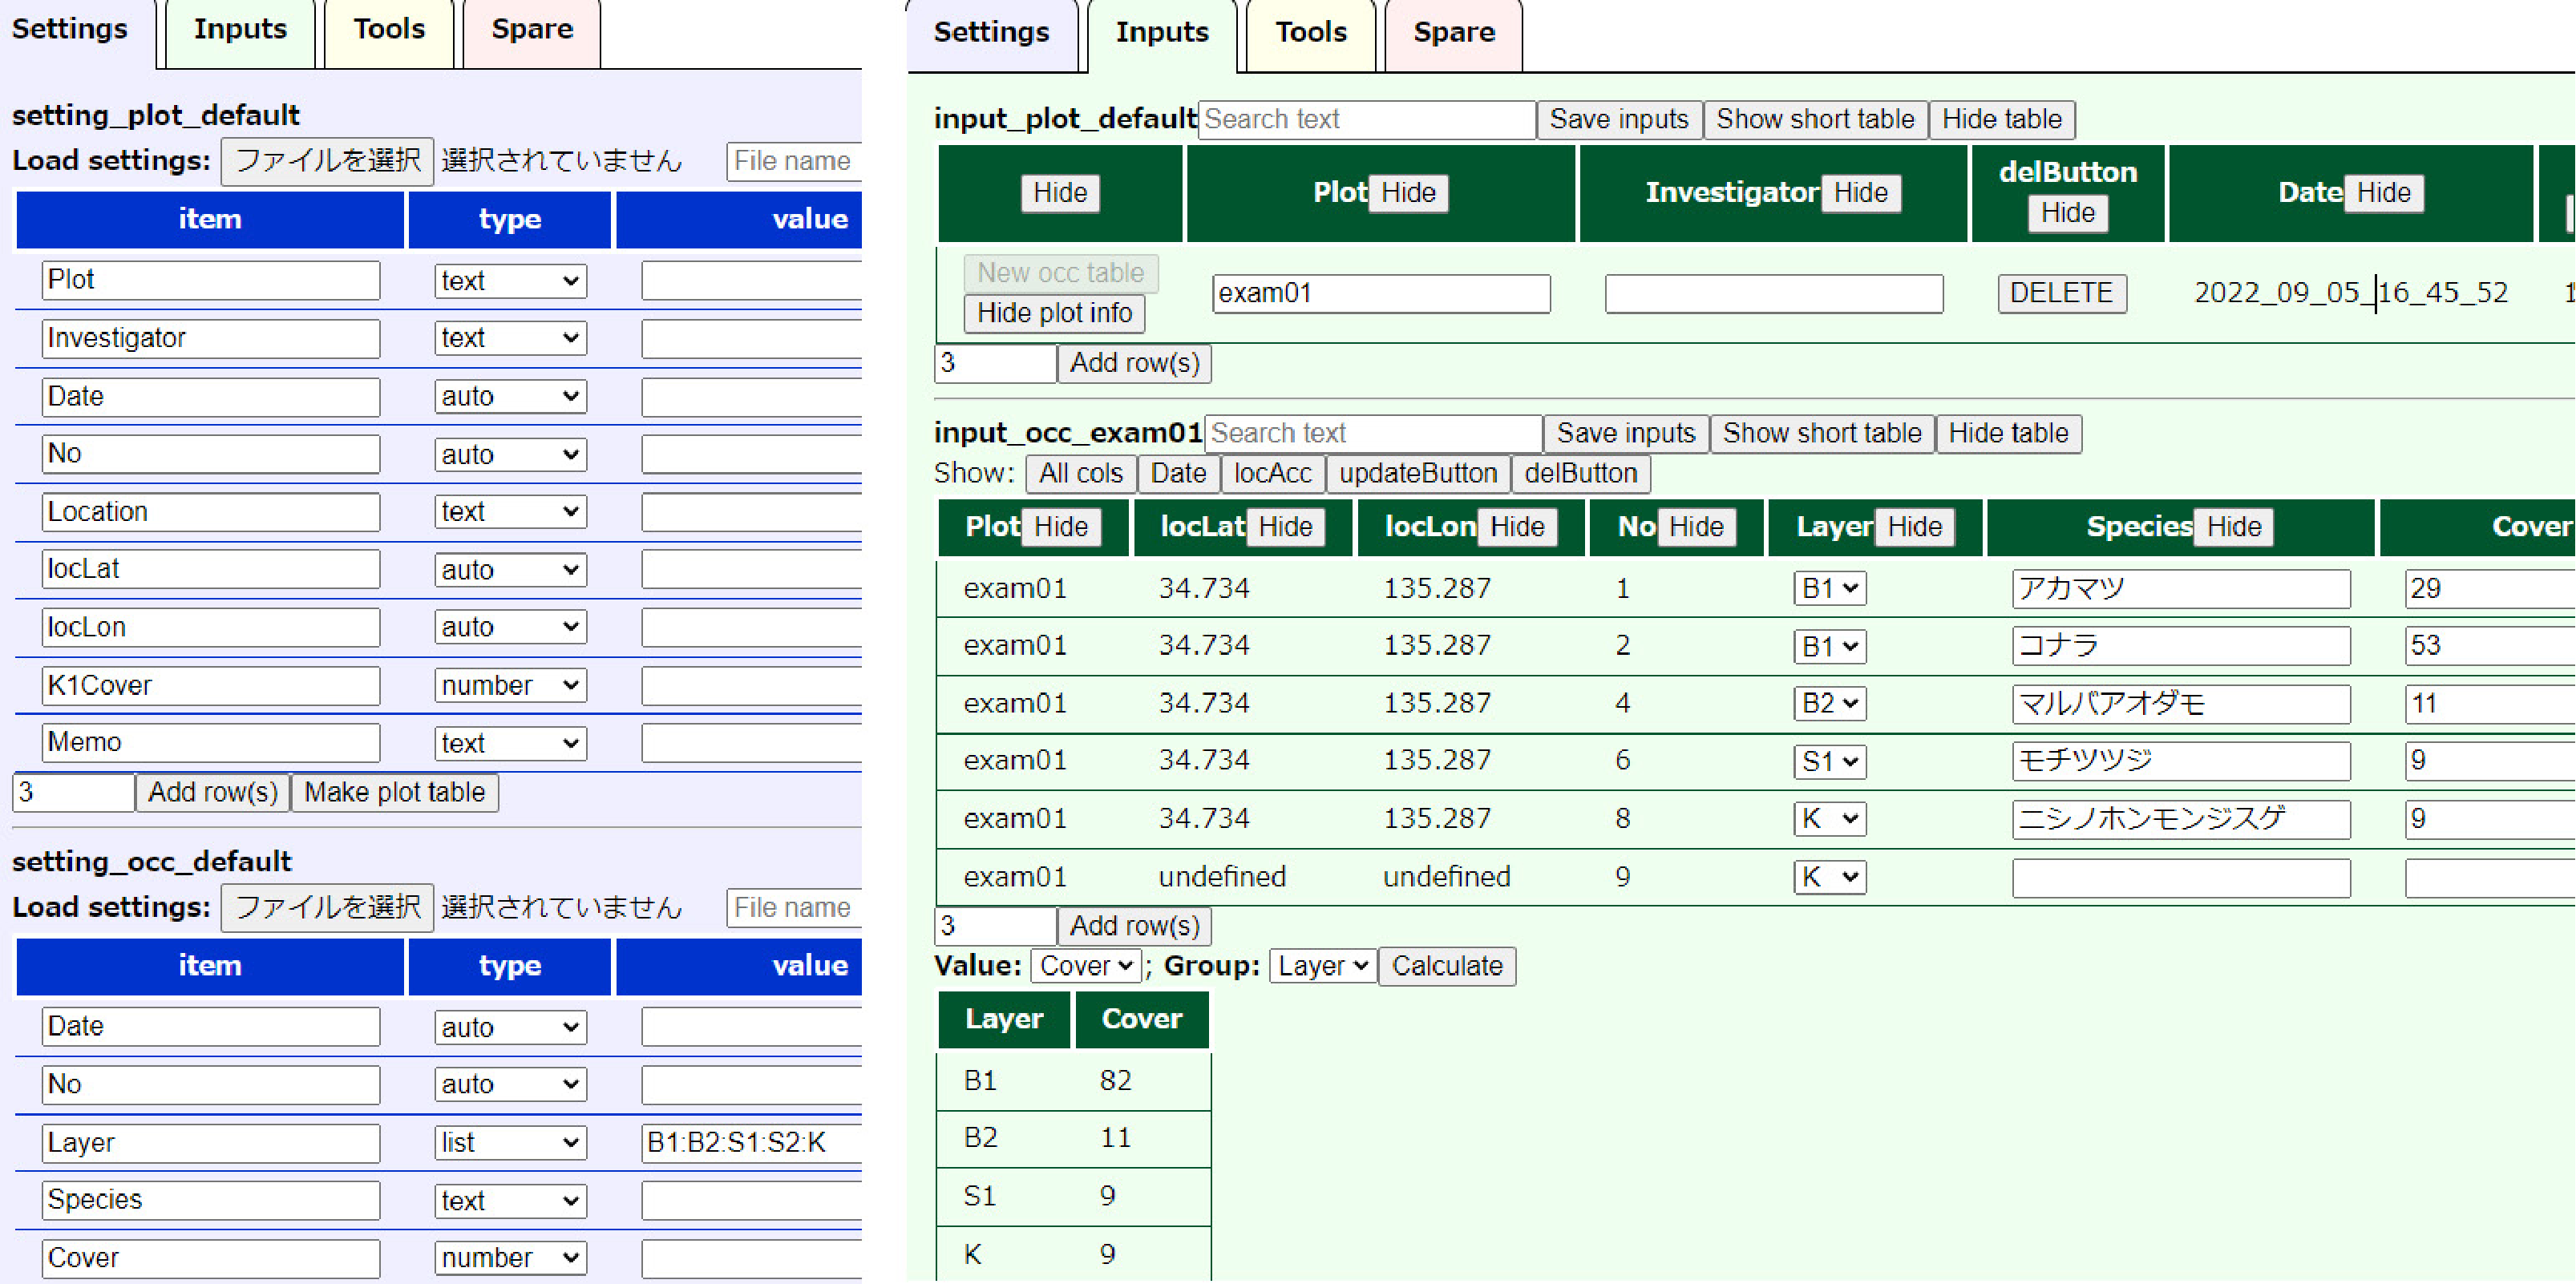
\includegraphics[height=63mm]{images2.pdf}

\includegraphics[width=20mm]{qr_code.pdf}

  % https://github.com/matutosi/ecan

\end{document}


  % ダミーのテキスト1
  % ダミーのテキスト2
  % ダミーのテキスト3
  % ダミーのテキスト4
  % ダミーのテキスト5
  % ダミーのテキスト6
  % ダミーのテキスト7
  % ダミーのテキスト8
  % ダミーのテキスト9
  % ダミーのテキスト10
  % ダミーのテキスト11
  % ダミーのテキスト12
  % ダミーのテキスト13
  % ダミーのテキスト14
  % ダミーのテキスト15
  % ダミーのテキスト16
  % ダミーのテキスト17
  % ダミーのテキスト18
  % ダミーのテキスト19
  % ダミーのテキスト20
  % ダミーのテキスト21
  % ダミーのテキスト22
  % ダミーのテキスト23
  % ダミーのテキスト24
  % ダミーのテキスト25
  % ダミーのテキスト26
  % ダミーのテキスト27
  % ダミーのテキスト28
  % ダミーのテキスト29
  % ダミーのテキスト30
  % ダミーのテキスト31
  % ダミーのテキスト32
  % ダミーのテキスト33
  % ダミーのテキスト34
  % ダミーのテキスト35
  % ダミーのテキスト36
  % ダミーのテキスト37
  % ダミーのテキスト38
  % ダミーのテキスト39
